\chapter{Results and discussion}
\label{sec:results}
\epigraph{Que tanto de peça para dar defeito.\\{\footnotesize (That's a lot of parts to malfunction.)}}{- My grandfather about my father's new car}

\begin{sidewaysfigure}[p]
    \AddThispageHook{\thispagestyle{empty}}
    \caption{Component maps and work line of the VT-80 engine}
    \label{fig:wline}
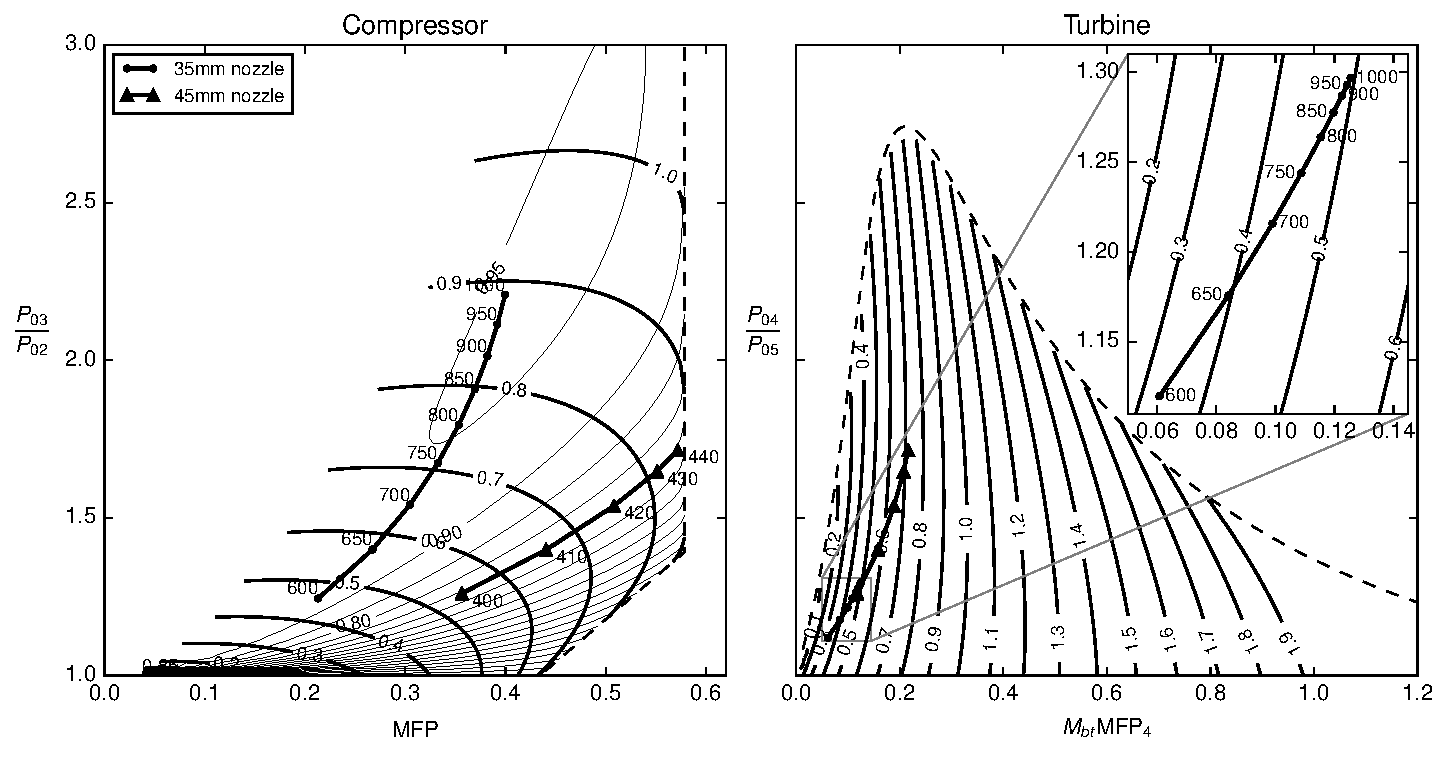
\includegraphics{fig/wline.pdf}
    \source{author's figure}
    \legend{Compressor and turbine maps for the VT-80 engine, with the work lines superimposed (thick line).
    The medium thickness contours are of constant blade Mach number and the thin contours are of constant polytropic efficiency. 
    Two working lines are shown: one for the actual turbine nozzle with 45mm diameter and another for a redesigned nozzle with 35mm diameter. 
    They are labeled with the turbine inlet stagnation temperatures ($T_{04}$), in kelvin.
    The surge line is not explicitly shown, and is the limit where the isospeed lines become undefined to the left hand side of the figure.}
\end{sidewaysfigure}


\Cref{fig:wline} shows the compressor and turbine maps and the work lines for
two nozzles: the actual 45mm nozzle and a redesigned 35mm nozzle.  The
compressor map is very in line with what is expected. Iso-rotation lines peak
slightly to the right of the surge line and then fall steeply towards the choke
line. Choke occurs in the compressor exit for pressure ratios bellow
approximately 1.4, as shown by the sloped choke line. There is a region of high efficiency near the surge line and
efficiencies fall for high mass flows and low pressure ratios. The turbine map,
on the other hand, is not what is typically found in the literature. This
happens because this turbine chokes at its exit in almost all operating
conditions. This leads to the iso-speed lines only becoming vertical near the
peak expansion ratio, and the choke line not being horizontal. 
The turbine was considered isentropic, so there are no iso-efficiency lines on its map.

Normally, well designed turbines choke on their inlets, and stay choked for most of the working range.
This helps to extract maximum work from the fluid and also reduces the turbine operating range. 
In order to achieve an inlet choke with this turbine, its inlet area should be severely reduced.

The nominal working line, with the 45mm nozzle, shows that there is a poor match between compressor, turbine and nozzle.
The compressor, in particular, is operating at quite low efficiencies and chokes with a very low value of $T_{04}$. 
Reducing the exit area of the nozzle by 10mm proved an easy way to increase its efficiency and avoid the choking region, while still keeping a good surge margin. 

To sum up, following design recommendations can be made based on the analysis of the component maps and work lines in \Cref{fig:wline}:
\begin{enumerate}
    \item the nozzle exit diameter should be reduced to 35mm, and
    \item the turbine areas should be redesigned. The inlet area should be made smaller so that it chokes in the design point, and the exit area should be made slightly larger than the inlet, to allow inlet choke and keep velocities approximately constant throughout the turbine.
\end{enumerate}

Off course, the efficiencies are grossly overestimated in this model. Further refinements might change some of these remarks.

\begin{figure}
    \caption{Flow state at each engine station}
    \label{fig:stations}
    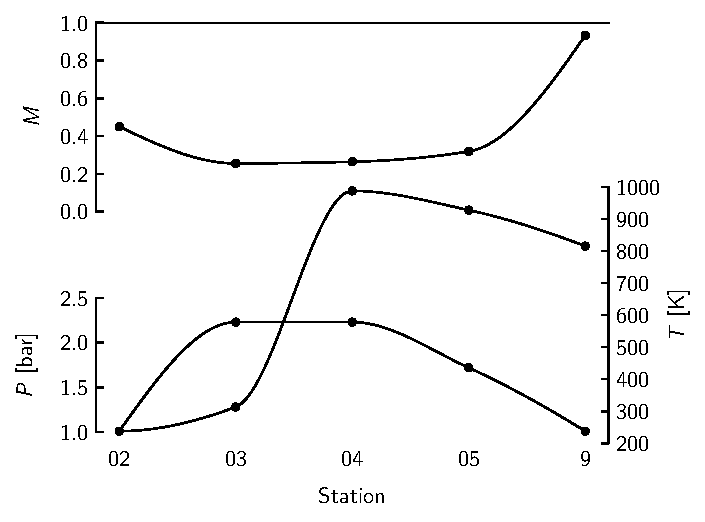
\includegraphics{fig/stations1000K}
    \source{author's figure}
    \caption*{Temperature, pressure and Mach number for each engine station at a turbine inlet temperature of 1000K and flight Mach number zero, using the redesigned 35mm nozzle. The temperature and pressure scales were chosen to keep their ratios to the reference values $\mathsf P_{01}$ and $\mathsf T_{01}$ comparable. When the station number is prefixed with a ``0'', the properties are from stagnation, otherwise they are static. Interpolation was done with the PCHIP algorithm \cite{Fritsch1980}, to keep lines smooth while not introducing artificial maxima.}
\end{figure}

\Cref{fig:stations} shows the temperatures, pressures and Mach numbers for each engine station at a reference turbine inlet temperature of 1000K and using the redesigned 35mm nozzle.
Again, it shows that the turbine inlet is very far from choke. This is a serious design flaw. The redesigned nozzle is almost choked in this condition, which is what is desired. Perhaps it could be made even narrower, to increase its Mach number to unity and thus generate more thrust. This, however, would decrease the surge margin.


\begin{figure}
    \caption{Comparison of model and experimental data}
    \label{fig:experimental}
    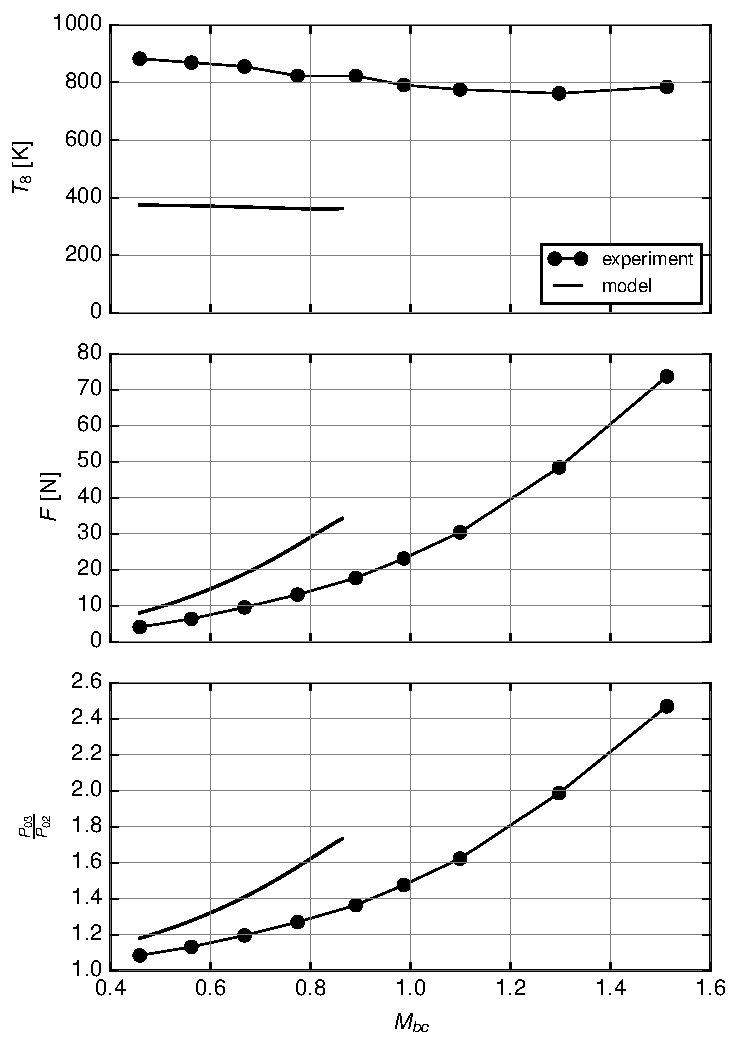
\includegraphics{fig/experimental}
    \source{\authorsfigure}
    \caption*{The performance predicted by the semi-empirical model data matches qualitatively well with the experimental data. The error is probably due to the overly optimist efficiency of the model components. The model data is only available up to the engine inlet choke. Experimental data was obtained by \textcite{bolsoni_test}.}
\end{figure}

\Cref{fig:experimental} shows a comparison of the engine model (considering the installed 45mm nozzle) and experimental data obtained in a test bench by \textcite{bolsoni_test}. In a qualitative analysis, the curve shapes are quite similar. Pressure ratio and thrust rise with the square of spool speed and exhaust gas temperatures are flat for both cases. The large quantitative difference in this temperature between model and experimental data is explained by the very low $T_{04}$ of the model, as can be seen in \Cref{fig:wline}. Even them the model shows greater thrust and pressure ratio. This is due to the very high efficiency considered by the model, since many losses were not included.

